\chapter{Toward a computational CMZ model comparison framework}
\label{chap:SMMEoutro}
\section*{Synopsis}
\textit{(1) The SMME introduces a phased structure in order to explain early RGC generation by \textit{Danio} RPCs, which is why it misapplies the explanatory logic of Gomes et al. \cite{Gomes2011} (2) A general-purpose statistical approach to testing many different kinds of models is desireable, and available in nested sampling. (3) Models of RPC activity in the postembryonic CMZ should prioritise simplicity, which could be achieved with ``slice models''. (4) Applying nested sampling to these models allows us to compare their explanatory quality rigorously.}

\section{SMME Postmortem: a wrong turn at Gomes}
To return to the question posed in \autoref{sec:SMMEexplanatorystrat}: has the SMME succeeded in finding order by blurring out the chaotic welter of mechanistic explanations for RPC function in retinogenesis? \autoref{chap:SMME} argues the structure of the SMME models support explanations based on the original idea of a linear, deterministic series of stages through which RPCs progress, originally put forward by Cepko et al. \cite{Cepko1996}, rather than stochastic processes. The important feature of the SMME models is where they depart from the original Gomes SSM: the assumption of the linear structure of temporal phases. The succession of stages is the model ingredient that produces the structure resembling the data, not the various random variables associated with mitotic mode, which we have proven by demonstrating that a deterministic progression of mitotic mode models the observations better than its stochastic counterpart. By introducing variability into the lengths of the linear temporal program already assumed by the SMME models, we can remove variability from the mitotic mode and produce a superior model with fewer parameters. Only by the process of counterinduction \cite{Feyerabend1993}, the comparison of models with different propositional structures about reality, does this become clear. The introduction of the linear phase structure is required to model the early contribution of RGCs in zebrafish. If this is left without some biological rationale, retinogenesis remains unexplained. The SMME thus does not achieve its aim of being a complete description of lineage outcomes in retinogenesis, and this is confirmed by our observation that the Wan model \cite{Wan2016} has little explanatory power outside the first few days of life, which makes up a small portion of the total retinal contribution to the zebrafish retina.

The first theoretical maneuver of the SMME, explaining the data with a model with structure that supports a stochastic mitotic mode process, cannot be achieved. The underlying data used to inform these models speak better to an entirely different selection from the array of theoretical options outlined in \autoref{sec:TheoryOptions}, the linear progression of competencies. Because the SSM model form does not usually have spatial dimensions, we did not test models involving variablility in extracellular signals, but it is a good bet that such a model could be made to fit about as well as either of the ones tested in the previous chapter. In effect, if we are to follow the SMME's inferential logic, variability in RPC outcomes can be explained by ``stochastic variability" in any model parameter which affects fate outcomes. Because of the significance of this problem for biological inferences, an explanation of the Bayesian epistemological view of probability has been provided in \autoref{ssec:BayesEpistemology}. Moreover, a thorough argument that ``stochasticity'' cannot be a property of real existents is provided in \autoref{sec:chance}. It suffices here to conclude that the SMME models do not achieve the aim of supporting ``stochastic processes'' as explanations over the alternatives.

The second theoretical maneuver, to nominate a particular macromolecular system as the physical locus of the stochastic process, suggests Atoh7 and Ptf1a as labels for abstract, Bernoulli distributed processes. It remains obscure how model variables relate to their namesake transcription factors (transcription of the TF itself? activation of other genes?), and no measurements of these factors inform parameter selection. Plainly, these factors are involved in relevant RPC behaviours, but it is unclear why they have been nominated as causally upstream of the ``mitotic mode'' selection. Since the Boije model inherits the assumption of a linear progression of stages, it is very likely that a model with similar explanatory power could be built using the same strategy outlined above, locating random variability outside mitotic mode, although this is outside the scope of the present work.

We conclude that the sole formally testable model of RPC function in the zebrafish retina is not adequate for our purposes. But how did we get here? As noted in \autoref{Raff}, the notion that the most significant behaviours associated with RPCs are produced by mechanisms intrinsic to the cells derives much of its empirical support from the Raff group's work. This story began with the observation that co-culturing E15 rat RPCs in dissociated pellet cultures with P1 cells did not accelerate the appearance of the first rods derived from the E15 progenitors (which occurred at a similar time as \textit{in vivo}), suggesting a partially intrinsic commitment ``schedule" for these cells\footnote{Co-culturing with P1 cells, did, however, significantly increase the proportion of E15 RPCs specified as rods, resulting in Raff's suggestion here that both intrinsic and extrinsic factors are important.} \cite{Watanabe1990}. The scope of these observations were dramatically expanded by Raff's subsequent work, intended to address the relative significance of intrinsic versus extrinsic processes in RPC function by comparing clonal RPC lineages in fully dissociated clonal-density cell culture to those in intact explants \cite{Cayouette2003}. The remarkable finding of this study was that dissociated E16-17 rat RPC lineages produce very similar numbers and types of retinal neurons as their tissue-embedded counterparts, albeit without morphological or molecular markers of mature neurons. This observation provided strong evidence for the predominance of RPC-intrinsic processes in determining both mitotic and fate outcomes for late RPC lineages. The complex, spatially organised context of intact explanted tissue seemed to only be required for the maturation of neurons, and was not required to regulate proliferation, or the initial commitment to an appropriate distribution of lineage outcomes. As correct cell numbers and types are the two most important parameters that must be controlled for RPCs to produce a functional retina of the appropriate size, the suggestion that both are largely determined by intrinsic processes seemed to confirmation of Williams and Goldwitz's much earlier suggestion \cite{Williams1992}, against the prevailing view of the day, that lineage had a greater role to play than cellular microenvironment in RPC contributions. Interestingly, Raff's interpretation of their 2003 data was that RPCs were most likely stepping through a linear, programmed developmental sequence, rather than undergoing shifts in the probabilities of variable outcomes over time. It is notable that this interpretation arises not from the data collected in their study, but from considerations of a single unusual clone reported by \cite{Turner1990}, and by analogy with drosophila neuroblasts. In retrospect, these arguments for linear sequences of deterministic RPC outcomes do not seem particularly strong, and it is perhaps unsurprising that these studies are remembered mainly for highlighting the importance of RPC-intrinsic processes.

The Gomes study, with its detailed study of particular rat late-embryonic RPC lineages, thus seemed to solidify the notion that unpredictable RPC-intrinsic processes dominate lineage outcomes \cite{Gomes2011}. But this study, like its forebears originating in Raff's work, is concerned with a population of RPCs that is too old to produce RGCs. This is the essential point: the SMME does not try to explain the early appearance of RGCs in terms of some macromolecular mechanism, although this is the single most significant difference between the zebrafish RPC lineages studied by Harris and the rat lineages studied by Raff and Cayouette \cite{Cayouette2003, Gomes2011}. It is only by assuming the unexplained linear temporal structure of RPC specification that the SMME models achieve their apparently good explanatory quality.

\section{Implications of the SMME study for modelling CMZ RPCs}
Having taken seriously the possibility that an adequate model of zebrafish retinogenesis already exists, and concluded in the negative, we may ask how to improve on this state of affairs. Firstly, careful model estimation is needed, and to have any confidence about our interpretation of the model, we must test alternatives that make different assumptions about the causal structure of the phenomenon being explained by the models. Can we conclude that the approach used in \autoref{chap:SMME} is adequate to our task? There are two elements to consider: the appropriateness of the modelling approach represented by the SSM in relation to the hypotheses we wish to test, as well as the soundness of the statistical procedures.

Taking up the SSM, its most attractive features are its computational efficiency and the ease of producing a model to fit some particular case-  the SMME models include some elements like the correlation of cell cycle lengths in mitotic sisters that greatly improve the temporal modelling of RPC lineage outcomes, for instance, which we will adopt in simulations presented below. The observations arising from the SMME strongly suggest that we would like to test hypotheses about RGC specification in order to find better models of RPC function. Carefully reconsidering the hypothesis of Neumann et al. \cite{Neumann2000}, that Shh from nearby RGCs induces cell cycle exit and RGC specification, would seem to be a high priority, for instance. Can such a scenario be represented in an SSM? One could model the probability of being within Shh induction range of an RGC in the early part of a lineage's life, for instance. Doubtless, a model that incorporated variable RPC specification outcomes determined on this basis could be made to fit data about as well as the variable mitotic mode or variable phase length models tested above. That said, it is not very clear that a highly abstract representation of signalling would constrain the inferred RGC production rate well. Moreover, while we showed that our deterministic mitotic mode model fit test data somewhat better than the stochastic model, the modest size of the calculated AIC differences suggests that comparing SSMs is not a particularly good way to distinguish even alternative hypotheses about the structure of processes the SSM models explicitly, like cell cycle length and mitotic mode. 

It seems that we will be unable to test important models, including those involving documented macromolecular explanations of RGC specification, without the ability to represent some spatial information. Still, the computational benefits of the SSM are too appealing to leave out of the toolkit entirely, and the type of spatial information that is ultimately best used to constrain alternatives on processes like RGC fate commitment could be highly abstract. We would like to leave the door open for models of many forms, prioritising simpler ones. Taken together, this suggests that we need a very general method of testing models of potentially very different structures against one another.

Turning then to our statistical procedures, are these adequate to our goals? We can broadly characterize the approach taken as estimating the local optimum of a loss function for model output, given the dataset; specifically, minimizing \hyperref[ssec:AIC]{Akiake's information criterion} by \hyperref[ssec:SPSA]{simultaneous perturbation stochastic approximation (SPSA)}. This procedure has some advantages. AIC is a well-understood measure, well-grounded in information theory, which penalizes superfluous model complexity in a consistent and rigorous way. SPSA is a widely used, well understood algorithm that can be applied to any reasonable euclidean parameter space; cases where parameter spaces are bounded (typical of biological models where negative parameter values are usually nonsensical) are explicitly accounted for, and so on. This procedure is better than many that are available.

Still, after the experience of the SMME model comparison, caution is warranted. The AIC calculation is based on a single estimate for the locally optimal parameterisation of the model. Relative AIC rankings are strongly influenced by the "well depth" of the AIC surface at the local minimum in parameter space\footnote{These problems are discussed in more detail in \autoref{ssec:AIC} and \autoref{ssec:overfit}.}. Indeed, blind interpretation of AIC rankings has lead to its use in ecology being described as a "cult" \cite{Brewer2020}. It is easy to imagine practitioners being reduced to "AIC hacking", in the same manner that "p hacking" occurs, in order to achieve some arbitrary value for a hypothesis.

Moreover, while SPSA is a practical algorithm its statistical guarantee is only that it will almost-surely find the local minimum of the loss function. For highly parameterised models with complex loss function surfaces, there will be many local minima for SPSA to get "stuck" in that are far from the global optimum\footnote{This is part of what is meant by "the curse of dimensionality", when speaking of the difficulty of sampling the loss function in high dimensional parameter spaces.}. If we are evaluating hypotheses in order to make decisions about potentially years-long research projects, more certainty about the reliability of the method is necessary. Finally, while SPSA is requires much less computational effort than more global Monte Carlo parameter estimation techniques like simulated annealing or Hamiltonian Monte Carlo, it requires about as much application-specific tuning.

Fortunately, a complete system of Bayesian inference, which addresses all of the problems mentioned above, has been promulgated over the last 15 years: nested sampling. Originally introduced by John Skilling \cite{Skilling2006}, this use of this system has became widespread in cosmology \cite{Trotta2008,Feroz2009,Higson2019}, where its generality and ability to cope with complex, high dimensional parameter spaces has been well proven. This system is discussed in detail in \autoref{ssec:nested}. We have implemented two separate samplers for the exploration of parameter spaces using the overall nested sampling approach: \path{GMC_NS.jl}, described in \autoref{chap:GMC}, and \path{BioMotifInference.jl}, described in \autoref{chap:BMI}. \path{GMC_NS.jl} is a prototype general purpose Galilean Monte Carlo sampler intended to perform nested sampling of arbitrary tissue- or cell-level biological models, while \path{BioMotifInference.jl} is a highly specialized, well-tested, ad hoc sampler for evidence calculation and MAP estimation of \hyperref[ssec:ICA]{independent component analysis} models of genetic sequence emission. \path{GMC_NS.jl}, while less mature, is of greater general interest, and having it in hand allows us to broadly consider the features of CMZ models we might like to test, before proceeding to test the function of the package and to determine its general utility in tissue-scale models.

\section{CMZ models in a putative model comparison framework}
The simulations presented in \autoref{chap:SMME} consisted solely of abstract collections of lineages. The members of these model colonies have no activities beyond proliferation, and no functional attributes beyond their proliferative status\footnote{I.e. the specified identity of post-proliferative cells in these models has no function within the model.}. Despite the underlying code consisting of relatively high performance C++, these simple models nonetheless occupied the \hyperref[sec:cluster]{local component of the cluster used in this work} for more than a week. Because the introduction of explicit three-dimensional spatial simulation implies much more computational expense, this could strongly limit the ability to test inferences with local resources. This constraint dominates other considerations in building models of the CMZ. Since funding constraints limit the cloud-export of computational burden from the confines of the research institution, it is reasonable to proceed upwards in model computational expense, seeking the minimum model complexity required to compare hypotheses of interest to us.

\subsection{Spatial dimension of the models: the "slice model"}
\label{ssec:slice}
Although decomposing the RPC population of the CMZ into a collection of unordered, independently-proliferating SSMs prevents us from assessing many interesting hypotheses, a computational model of the entire CMZ or retina may not be required. Because observations suggest that RPC lineages contribute to the retina in linear cohorts of neurons, any particular centrally-oriented slice of the CMZ annulus will be responsible for the generation of the neurons central to it. The retina can represented by a series of these "slice units", lined up radially, like slices of pie. A complete "slice unit" would include the central-most larval remnant, contributed by embryonic retinogenesis, surrounded by the CMZ's more ordered neural contribution from the postembryonic period, and, peripherally, the CMZ itself. Depending on the hypotheses to be tested, the differentiated central retina may be mostly irrelevant, so the modelled slice may consist only of the CMZ and its interface with these central neurons. It is important to note that these slices are conceptually different from the linear cohorts generated from particular lineages, the so-called `ArCCoS', which justify the slices conceptually \cite{Centanin2011}. It is not necessarily the case that a slice model would consider only one RPC lineage; the slices are better thought of as spatial boxes that sample the CMZ, the conceptual equivalent of the histological section through the eye\footnote{The case of only one simulated lineage may still arise given thin enough sample boxes or old enough animals, but it is a limiting case and probably would not be the norm.}.

\begin{figure}[!h]
    \makebox[\textwidth][c]{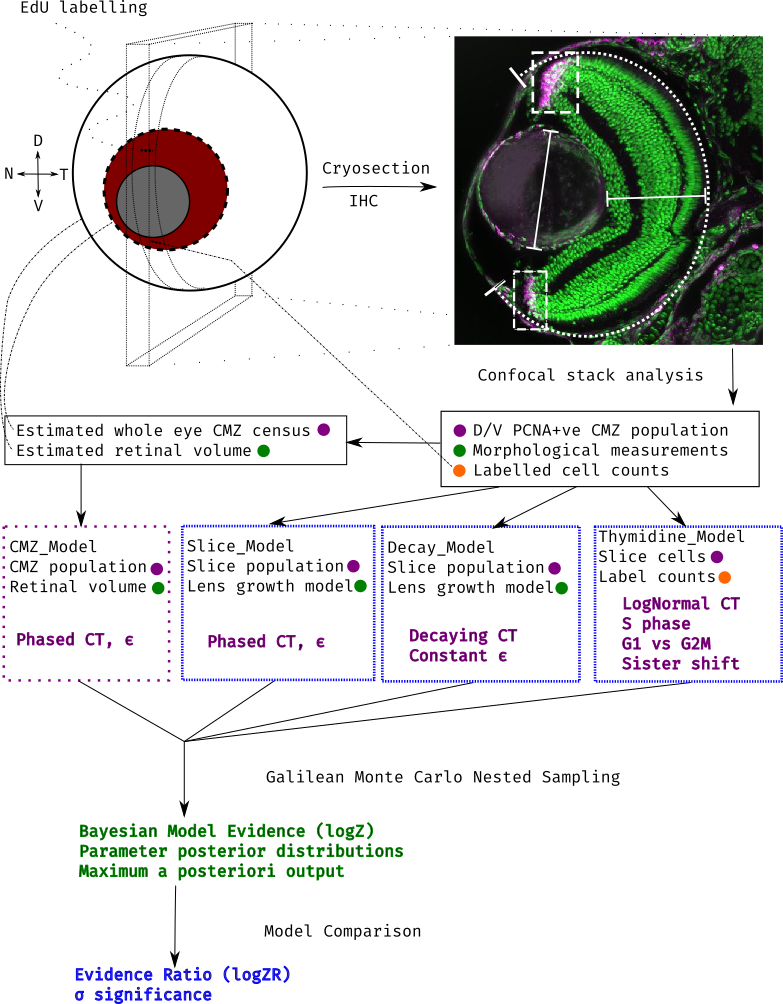
\includegraphics[width=0.85\textwidth]{cmz/slice.png}}    
    \caption{{\bf Whole-eye and slice model abstractions of CMZ RPC populations used in \autoref{chap:CMZ}}}.
    \label{cmzslice}
    D/V: Dorsoventral axis. N/T: Nasotemporal axis. Red torus: CMZ. Grey circle:Lens. Colored dots denote the data sources used in each model. Magenta text gives the parameters of the model. CT: Cycle time. $\epsilon$: exit rate. See \autoref{chap:CNS} for more.

    Data to estimate models were acquired from immunohistochemical analyses of cryosections through \textit{Danio} eyes. Confocal stacks were segmented and analysed to count PCNA+ve and (if applicable) EdU-labelled CMZ cells in the slice as well as to measure the lens and neural retina. These slice data were used to estimate whole-eye measurements for a fully abstract \path{CMZ_Model}, representing the entire peripheral RPC population, as well as directly compared to the output of three different types of \path{Slice_Model}. Quality estimates from these models were sampled by GMC-NS, producing model evidence, posteriors, and MAP output. Model evidence was compared to produce estimates of the evidence ratio and significance.
\end{figure}


Slice models are especially attractive because the proliferative status, position, specified fate, etc. of simulated cells can be directly compared to measurements of fixed sections of retinal tissue. This is especially important for studying the postembryonic CMZ, which rapidly becomes optically inaccessible due to the increasing thickness and pigmentation of overlying tissue, so that live imaging often cannot be used \footnote{It is worth noting that the spatial parameters of such models would pertain to fixed and not live retinas; it is probable that some scaling relation compensating for fixative shrinkage could allow the mixture of live imaging data in evidence calculations.}.

If the retina can be thought of as a series of slice models, and the activity of the CMZ is basically homogenous around its circumference, the activity of the CMZ may be usefully represented with a single such model. Moreover, the slice need only include one portion of the retinal periphery, the orientation of which is irrelevant (i.e. the model parameterisation for the dorsal portion of a coronal slice could be identical to the ventral). It may be erroneous to abstract such a slice from its context, because the modelled cells are in contact with adjacent slices. In this thesis, in order to model the interaction between the simulated slice and the rest of the eye, we use a model of lens growth to produce an estimate of the number of additional fractional CMZ slices the modelled slice would have had to produce in order to maintain the CMZ annulus. The appropriate number of RPCs are subtracted from the slice's population, which models the lateral, slice-adjacent interface of the CMZ in addition to niche exit from the CMZ into the neural retina central to the CMZ slice. The various models used in \autoref{chap:CMZ} are summarised in an inferential pipeline schematic in \autoref{cmzslice}.

The zebrafish retina is a manifestly asymmetrical structure, with an optic nerve positioned ventro-temporally relative to the center of the optic cup. The CMZ itself is generally understood to be an asymmetric structure, with a larger dorsal than ventral population. This calls into question the assumption of CMZ homogeneity outlined above. It is nevertheless plausible that the appearance and maintenance of these structural features of the zebrafish retina could be explained with a set of slice models, for example, one for each of the dorsal, ventral, nasal, and temporal extrema\footnote{Such models are implemented by \hyperref[chap:CNS]{\path{CMZNicheSims}} as \path{MultiSlice_Models}.}. Ultimately, these considerations are only relevant if our objective is to compare model explanations for retinogenesis as a whole. If we restrict ourselves to the more modest goal ranking causal influences on the lineage outcomes of RPCs in the dorsal extremity of the CMZ, a slice model could still be valuable even if it fails to explain aspects of tissue-level zebrafish retinogenesis.

\FloatBarrier

\subsection{Temporal resolution of the models}
Another important consideration for any CMZ model comparison framework is the time-scale of any phenomena which are to be admitted as possible causal contributors to retinogenesis. While it is reasonable to think that proliferative events may be well-described with a model that operates on a scale of days and fractions thereof, and that such a model would be well suited to describing the full sweep of CMZ activity across the life of the organism, very few of the relevant macromolecular processes are likely to be well-described with a resolution more coarse than seconds or minutes. The implied difference in the number of calculations required to simulate any given time period is thus several orders of magnitude. A simplifying assumption of the temporal homogeneity of CMZ activity would allow us to abstract long developmental time frames; an explanation that pertains to a few hours can perhaps be extended without recalculation. 

If an assumption of temporal homogeneity proves inadequate, the functional structure of the simulation will be determined by this consideration. To illustrate this, consider a case where we wish to incorporate measurements of eye pressure, or membrane tension across the retina, as inputs into the proliferative activity of the CMZ, by way of progenitor cortical tension \cite{Winklbauer2015}. This would permit assessing whether modelling tissue-mechanical inputs to cellular activities allows us to extract additional information from our observations. If such physical model elements are to be included, the functions which relate physical parametric data to the proliferative behaviour of CMZ progenitors must not operate on a time scale too short to cover the period of interest. Suppose we are mainly interested in explaining the assembly of functional units of the mature, specified retina by the CMZ, from the first division of the presumed distal stem cell responsible for the unit to the determination of the last neuron of its functional column. If this process takes days, finite element approximation of cortical tension with a resolution small enough to capture important details of relevant cellular movements (e.g. interkinetic nuclear migration) will probably be too expensive to allow for effective application of Monte Carlo techniques, requiring thousands or millions of simulations per call of the model likelihood function.

The models in this thesis mostly are of very coarse resolution, because they model the CMZ over significant portions of the organism's life; the exception is the \path{Thymidine_Model}, which is a cell-based intended to model thymidine analogue labelling of cells passing through S-phase, and is not intended to model RPCs leaving the niche at all. The \path{Thymidine_Model} is also by far the slowest of the \hyperref[chap:CNS]{CMZNicheSims} to estimate.

\section{Structuring models under uncertainty}
The extent to which model simplifications are justified, and the types of phenomena that could be explained with these models, depend heavily on considerations that can only be informed by observations. As has been demonstrated in \autoref{chap:SMME}, the growth of the CMZ population cannot be explained by SMME models fitted to embryonic RPC activity. However, it remains unclear what sort of alternative structure is justified by observations, given our uncertainty about inferred parameters of the populations being measured. Because we have, in \path{GMC_NS.jl} a general method of comparing differently parameterised models against our observations, we can seek to select models from among alternatives on the basis of their total explanatory power for the observations, independent of the particular model structure or parameter values. Because this process also produces samples from the posterior distribution of the model's parameters, we are also able to account for our uncertainty on these parameters. This allows us to broadly answer the question of what sorts of hypotheses may be addressed by the conventional immunohistological techniques we have used thus far, and what changes to methodology or analysis may be necessary to produce data that adequately constrains models of interest.

Our general approach is to estimate model evidence over broad prior distributions on model parameters. We assume as little as possible about the processes underlying our results. The values used in these comparisons are the logarithm of the model evidence, logZ, also understood as the logarithm of the marginal probability of the model. Likelihoods and probabilities are often compared in ratios; evidence is the same, and since the logarithm of a ratio is the logarithm of the numerator minus that of the denominator, this log-ratio, logZR, may be calculated by subtracting the evidence of one model from another. This is discussed in more detail in \autoref{ssec:nested}. This general model-comparison logic is iterated to address most of the important hypotheses we test in the following chapters.